
Raspbian ist das offizielle Betriebssystem f�r den Raspberry~Pi. Es kann in zwei unterschiedlichen Varianten heruntergeladen werden. Man kann zwischen einer minimalen Version (Lite) oder einer Version mit grafischer Oberfl�che und vielen vorinstallierten Programmen w�hlen. Es wird in beiden F�llen mindestens eine 4~GB gro�e MicroSD-Karte ben�tigt. Man sollte aber, um Reserven zu haben, mindesten 8~GB verwenden.\\  
Zur Installation ben�tigt man ein beliebiges Linux System mit einem MicroSD-Kartenleseger�t. Die aktuelle Raspbian Version kann als Image-Datei von der Seite \url{https://www.raspberrypi.org/downloads/raspbian/} heruntergeladen werden. Bei dieser Anleitung wird Raspbian Stretch Lite verwendet.

\begin{console}
	wget --trust-server-names http://downloads.raspberrypi.org/raspbian_lite_latest
	unzip 2018-03-13-raspbian-stretch-lite.zip
	rm 2018-03-13-raspbian-stretch-lite.zip
\end{console}


\subsection{Etcher}

Das grafische Programm Etcher (\url{https://etcher.io}) kann zum �bertragen der Image-Datei verwendet werden. Es ist vor Allem f�r Anf�nger zu empfehlen, da beim Konsolenprogramm dd das Risiko besteht, dass Daten einer falschen Partition bzw. eines Laufwerks zerst�rt werden. Das Programm muss allerdings manuell installiert werden.     

\begin{console}
	wget https://github.com/resin-io/etcher/releases/download/v1.3.1/etcher-1.3.1-linux-x86_64.zip 
	unzip etcher-1.3.1-linux-x86_64.zip
	chmod +x etcher-1.3.1-x86_64.AppImage
	sudo mv etcher-1.3.1-x86_64.AppImage /usr/local/bin/etcher
	etcher &
\end{console}


Nach dem Starten wird danach gefragt ob eine Verkn�pfung zum Programm erstellt werden soll. Dies sollte man mit "`Yes"' beantworten. Danach kann man mit der Schaltfl�che "`Image"' die Image-Datei ausw�hlen. Ist nur ein m�gliches Ziel vorhanden, wird es bereits vorausgew�hlt, z.~B. die SD-Karte im Karten-Slot (/dev/memcblk0) oder im USB-Adapter (/dev/sdb). Sind mehrere m�gliche Ziele vorhanden, wird die "`Select Drive"' Schaltfl�che freigeschaltet. Dann kann ein Laufwerk manuell ausgew�hlt werden.

\begin{figure}[ht]
	\centering
	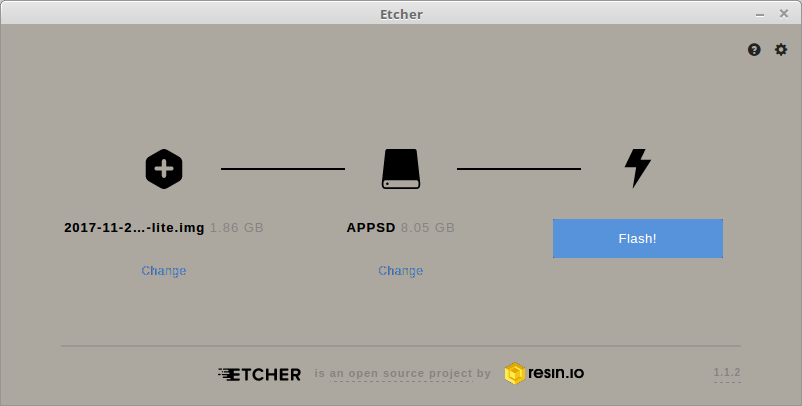
\includegraphics[scale=0.3]{images/Etcher_1.png}
	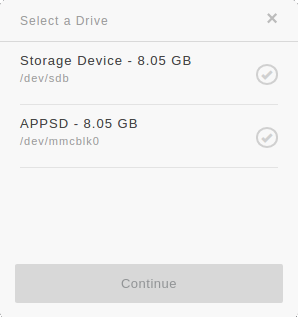
\includegraphics[scale=0.3]{images/Etcher_2.png}
	\label{Etcher}
\end{figure}


Wenn man noch etwas �ndern will, kann die entsprechende "`Change"' Schaltfl�che ausgew�hlt werden. Zum Schluss wird der Schreibvorgang mit der "`Flash!"' Schaltfl�che gestartet. M�glicherweise wird vom Programm allerdings noch das System-Passwort abgefragt.\\ 
Das Laufwerk bzw. die Partitionen werden nun aus dem System ausgeh�ngt und der Schreibvorgang gestartet. Der Fortschritt, die durchschnittliche �bertragungsrate und die Restlaufzeit werden w�hrend des Vorgangs angezeigt.\\ 


\subsection{dd Kommandozeilenprogramm}

Die erhaltene Image-Datei kann mit dem Kommandozeilenprogramm dd auf eine MicroSD-Karte �bertragen werden.\\
\textbf{Es ist unbedingt vor dem Ausf�hren des Befehls zu pr�fen, ob das angegebene Laufwerk bzw. Device auch der vorgesehenen MicroSD-Karte entspricht!}\\ 
Bei USB-Kartenlesern bzw. USB-Adaptern ist die Ermittlung des Devices leicht �ber die Systemmeldungen m�glich. 

\begin{console}
	dmesg | tail -n 10
\end{console}

\begin{screensmall}
	scsi 3:0:0:0: Direct-Access     MXT-USB  Storage Device   1308 PQ: 0 ANSI: 0 CCS
	sd 3:0:0:0: Attached scsi generic sg1 type 0
	sd 3:0:0:0: [sdb] 15730688 512-byte logical blocks: (8.05 GB/7.50 GiB)
	sd 3:0:0:0: [sdb] Write Protect is off
	sd 3:0:0:0: [sdb] Mode Sense: 03 00 00 00
	sd 3:0:0:0: [sdb] No Caching mode page found
	sd 3:0:0:0: [sdb] Assuming drive cache: write through
	sdb: sdb1 sdb2
	sd 3:0:0:0: [sdb] Attached SCSI removable disk
	EXT4-fs (sdb2): mounted filesystem with ordered data mode. Opts: (null)
\end{screensmall}

Die MicroSD-Karte wurde im Beispiel als Device "`sdb"' �ber einen USB-Adapter eingebunden. Nun kann man die Image-Datei mit dem Programm dd auf die MicroSD-Karte �bertragen. Mit dem Parameter "`of"' muss der komplette Device-Name, in diesem Fall "`/dev/sdb"', angegeben werden. Bei Parameter "`if"' wird die entpackte Image-Datei angeben. Die Bl�ckgr��e bzw. der Cache wird mit Parameter "`bs"' gesetzt. Eine gr��ere Blockgr��e erh�ht die Schreibgeschwindigkeit. Sie wird im Beispiel mit 4~MB angegeben.\\
Zu Beachten ist, dass der USB-Massenspeicher m�glicherweise bereits automatisch gemountet wurde. Dann sollte man die Partitionen mit dem Befehl "`umount"' zuerst auswerfen. 


\begin{console}
	umount /dev/sdb1 /dev/sdb2
	dd if=2018-03-13-raspbian-stretch-lite.img of=/dev/sdc bs=4M
\end{console}

\begin{screensmall}
	1323+0 Datens�tze ein
	1323+0 Datens�tze aus
	1387266048 Bytes (1,4 GB) kopiert, 127,6147 s, 10,4 MB/s
\end{screensmall}
